\begin{sidewaysfigure}
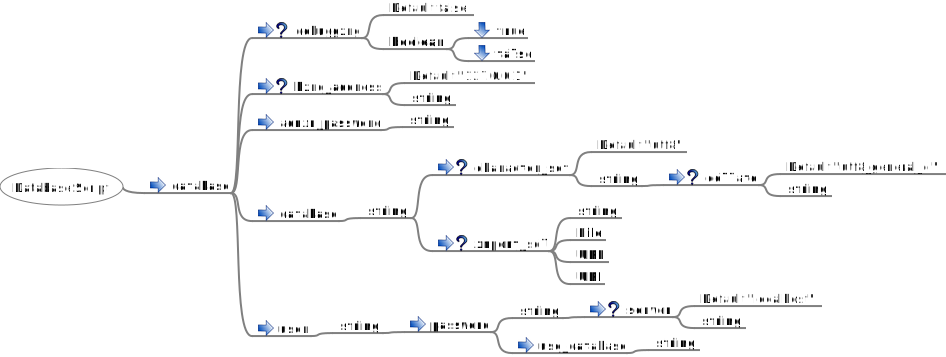
\includegraphics[width=0.9\textwidth]{database_service_script}
\label{fig:database_script_statements}
\caption{Database Script Statements}
\end{sidewaysfigure}

\begin{lstlisting}[style=Java,label=lst:database_ubuntu_profile,caption=Database Example Ubuntu Profile]
profile "ubuntu_10_04", {
    system {
        install_command "export DEBIAN_FRONTEND=noninteractive; /usr/bin/aptitude update && /usr/bin/aptitude install"
    }
    database {
        service "mysql"
        packages "mysql-server"
        configuration_directory "/etc/mysql/conf.d"
        restart_command "/etc/init.d/mysql restart"
    }
}
\end{lstlisting}


\begin{lstlisting}[style=Java,label=lst:database_example_script,caption=Database Example Script]
database {

    // enable debugging output
    debugging true

    // bind the database server to all addresses only
    bind_address "0.0.0.0"

    // set the administrator password
    admin_password "mysqladminpassword"

    // add new database with default character set and collate
    database "wordpressdb"

    // add new database
    database "drupal6db", character_set: "latin1", collate: "latin1_swedish_ci"

    // add new database and import tables
    database "maildb", {
        import_sql "postfixtables.sql"
    }

    // add new database and import tables
    database "postfixdb", character_set: "latin1", collate: "latin1_swedish_ci", {
        import_sql "postfixtables.sql"
    }

    // add a new user
    user "test1", password: "test1password", server: "srv1"

    // add a new user, grand all privileges on database
    user "drupal6", password: "drupal6password", server: "srv2", {
        use_database "drupal6db"
    }
}
\end{lstlisting}

\pagebreak

\begin{longtable}{lp{0.5\textwidth}}
\multicolumn{2}{l}{Commands Properties} \\*
\toprule
\endfirsthead
\endhead
\caption{MySQL Ubuntu 10.04 Properties}
\label{tbl:database_mysql_ubuntu_10_04_properties}
\endlastfoot
%
install\_command &
\code{/usr/bin/aptitude update \&\& /usr/bin/aptitude install} \\
%
restart\_command &
\code{/sbin/restart mysql} \\
%
mysqladmin\_command &
\code{/usr/bin/mysqladmin} \\
%
mysql\_command &
\code{/usr/bin/mysql} \\*
%
\toprule
%
\multicolumn{2}{l}{Files and Directories Properties} \\*
\toprule
%
configuration\_directory &
\code{/etc/mysql/conf.d} \\
%
mysqld\_configuration\_file &
\code{sscontrol\_mysqld.cnf} \\*
%
\toprule
%
\multicolumn{2}{l}{Other Properties} \\*
\toprule
%
packages &
\code{mysql-server} \\
%
default\_character\_set &
\code{utf-8} \\
%
default\_collate &
\code{utf8\_general\_ci} \\
%
\end{longtable}


